\documentclass{article}

\usepackage[english]{babel}

% Set page size and margins
% Replace `letterpaper' with`a4paper' for UK/EU standard size
\usepackage[letterpaper,top=2cm,bottom=2cm,left=3cm,right=3cm,marginparwidth=1.75cm]{geometry}

% Useful packages
\usepackage{amsmath}
\usepackage{graphicx}
\usepackage[colorlinks=true, allcolors=blue]{hyperref}

%\usepackage{caption}
%\usepackage{subcaption}
\usepackage{subfig}

\title{Preliminary Analysis of Stroke Participant's Movement}
\author{Milli Schlafly}

\begin{document}
\maketitle

Analysis notes:
\begin{itemize}
	\item Movement when the ball is green is removed. (Only matters for a couple participants)
	\item Movement when participant is not lifted is removed. (Negligible effect on results)
	\item Window of +/- 0.3Hz
	\item Statistics obtained with repeated measures ANOVAs
\end{itemize}

Ball frequency is a significant factor in nearly every ANOVA that was performed. Because this result could be due to factors other than the participant's ability to produce motion at the ball's resonant frequency, I do not note if ball frequency is significant in this document. 



\begin{figure}[!ht]
     \centering
     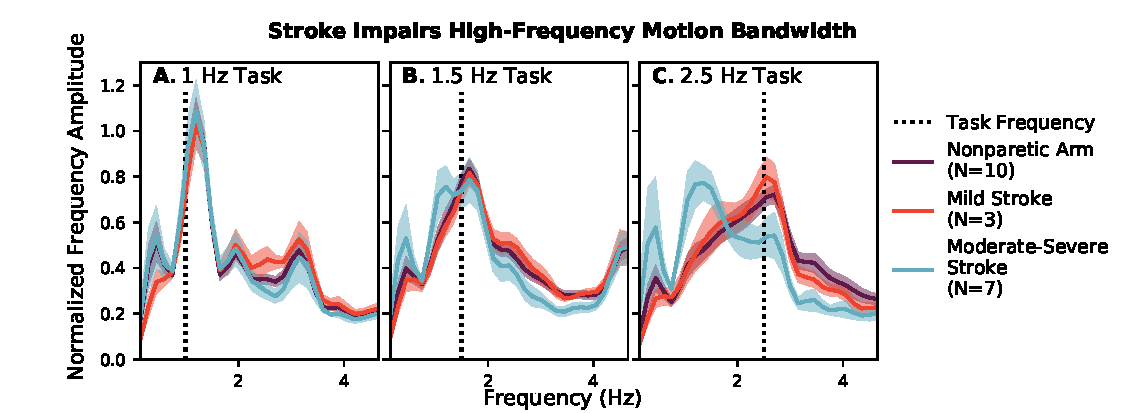
\includegraphics[width=\linewidth]{Plots/plots_combined.pdf}
	%\caption{}
\end{figure}


\section{Moderate-Severe Stroke Aggregate Results}

Included participants (N=7): Sub208 (FMA-37), S211 (FMA-17), S212 (FMA-13), S214 (FMA-32), S218 (FMA-7), S219 (FMA-7), S220 (FMA-21) 

\begin{figure}[!ht]
     \centering
     \subfloat{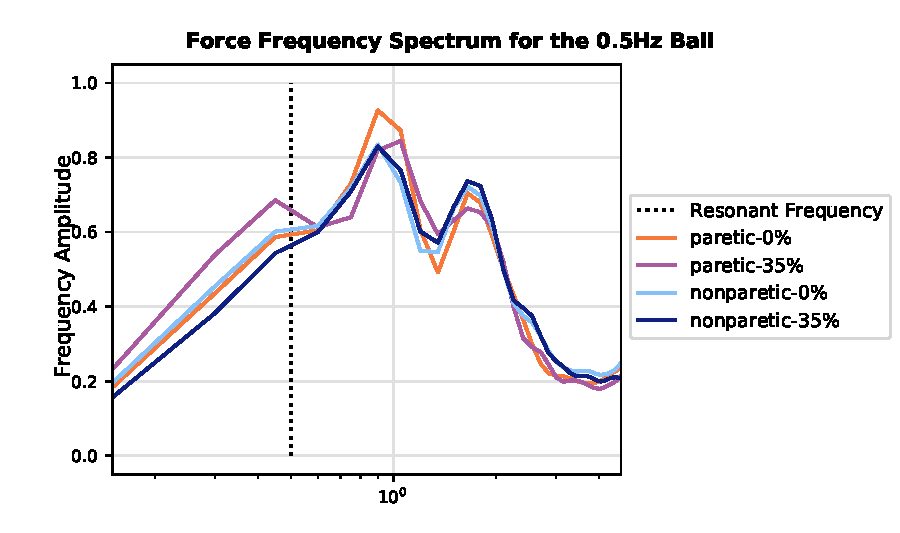
\includegraphics[width=0.49\linewidth]{Plots/agg_spectrum_0.5Hz_ms.pdf}}
     \subfloat{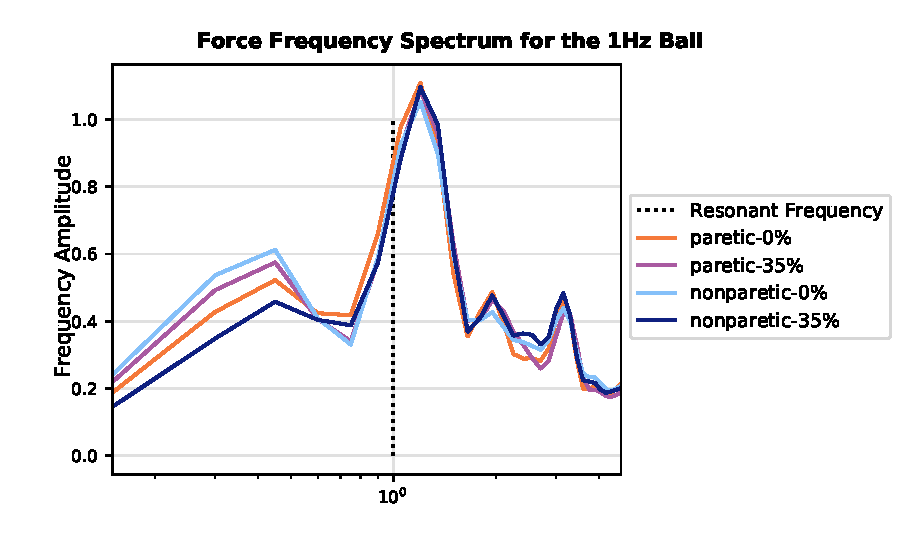
\includegraphics[width=0.49\linewidth]{Plots/agg_spectrum_1Hz_ms.pdf}}
     \hfill
     \subfloat{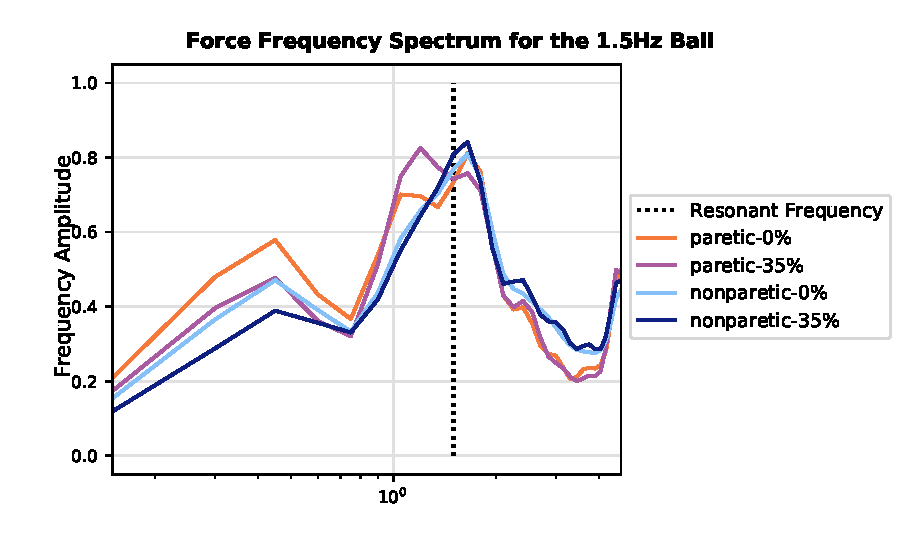
\includegraphics[width=0.49\linewidth]{Plots/agg_spectrum_1.5Hz_ms.pdf}}
     \subfloat{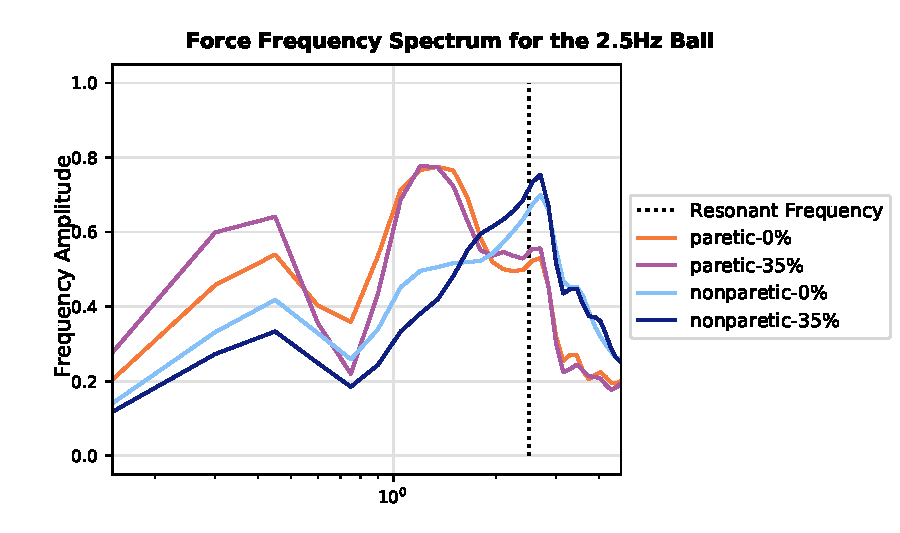
\includegraphics[width=0.49\linewidth]{Plots/agg_spectrum_2.5Hz_ms.pdf}}
     \hfill
	\caption{Aggregate Frequency Spectrums for participants with moderate-severe stroke. Trends are stronger than all participants combined. With the 1.5Hz and 2.5Hz ball, participants struggled to reach the resonant frequency with their paretic arm, resulting in a mound (or, for 2.5Hz, a second peak) below the resonant frequency. No trends are apparent at 0.5Hz.}
\end{figure}


\begin{figure}[!ht]
     \centering
     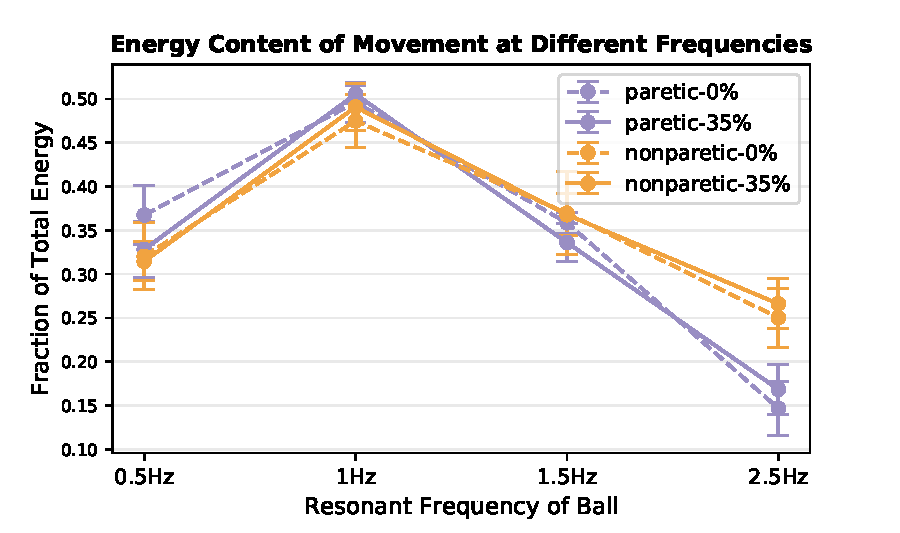
\includegraphics[width=0.49\linewidth]{Plots/e_at_res_raw_ms.pdf}
	\caption{Energy at the resonant frequency of the ball metric for participants with moderate and severe stroke. There is an interaction effect between arm and task frequency (p=0.02). Arm is not a significant factor for the 0.5Hz (p=0.14), 1Hz (p=0.82), and 1.5Hz (p=0.40) balls. For the 2.5Hz ball, arm is a significant factor (p=0.01). Loading is not significant in the paretic arm (p=0.13)---loading marginally improves performance at 0.5Hz (p=0.07) and hurts performance at 1.5Hz (p=0.33). It is harder to distinguish differences between loading and no loading at 2.5Hz because many participant struggles to even move at that speed.}
\end{figure}

\begin{figure}[!ht]
     \centering
     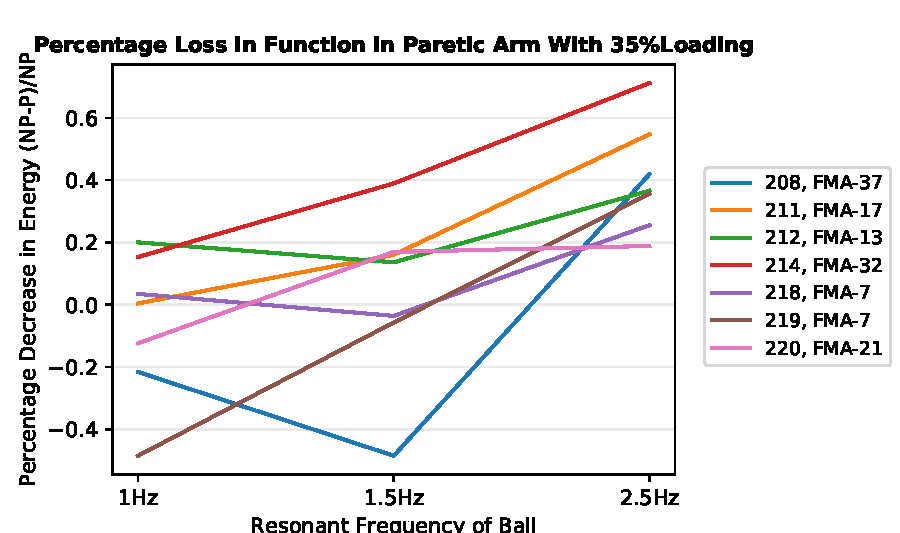
\includegraphics[width=0.49\linewidth]{Plots/pl_SL1_indiv_ms.pdf}
     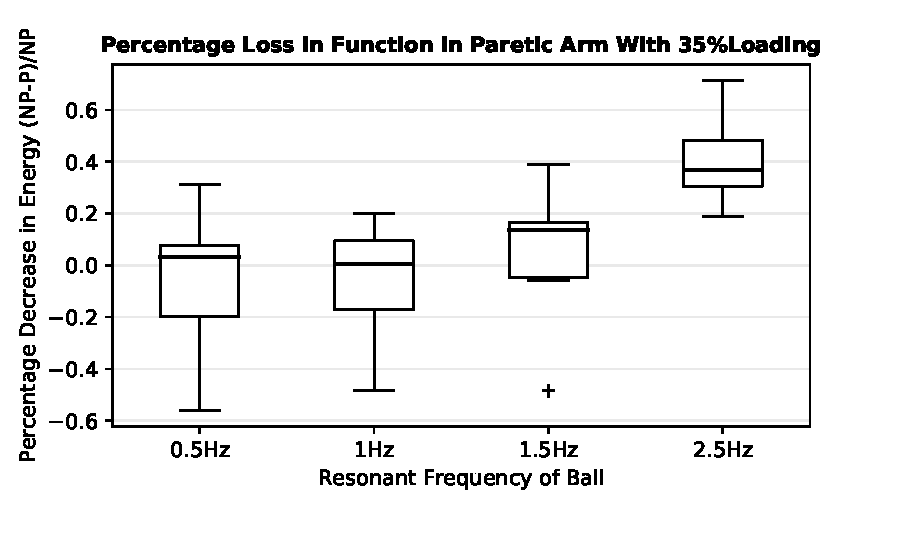
\includegraphics[width=0.49\linewidth]{Plots/pl_SL1_ms.pdf}
	\caption{Percent loss in paretic arm with loading in moderate and severe stroke. Positive values indicate better performance in the nonparetic arm. Negative values indicate better performance in the paretic arm. Ball frequency is significant (p=0.016) with energy at resonance using the 2.5Hz ball being different from the rest.}
\end{figure}

\begin{figure}[!ht]
     \centering
     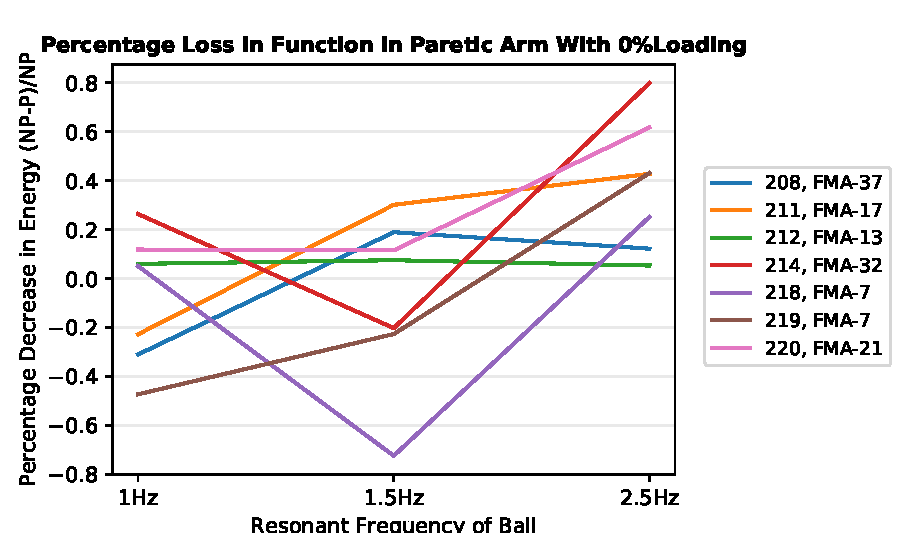
\includegraphics[width=0.49\linewidth]{Plots/pl_SL0_indiv_ms.pdf}
     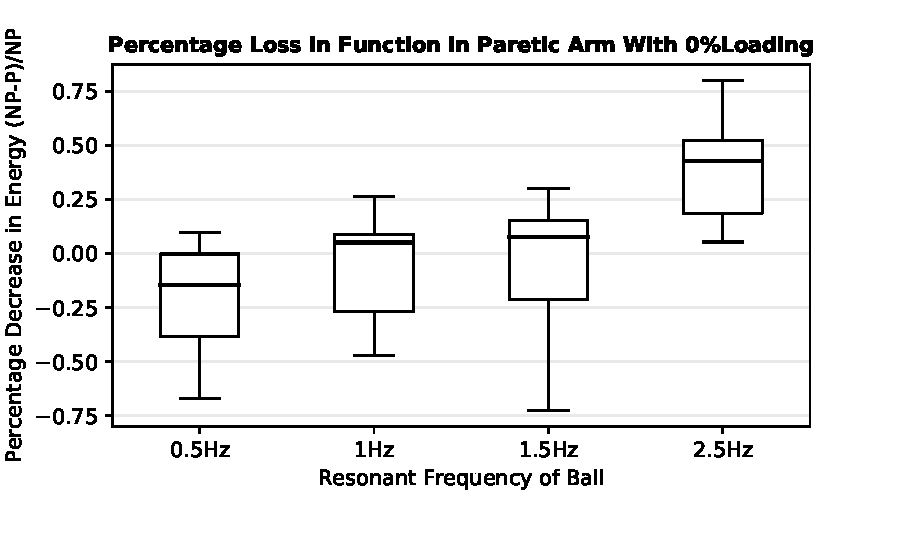
\includegraphics[width=0.49\linewidth]{Plots/pl_SL0_ms.pdf}
	\caption{Percent loss in paretic arm with no loading in moderate and severe stroke. Positive values indicate better performance in the nonparetic arm. Negative values indicate better performance in the paretic arm. Ball frequency is significant (p=0.019) with energy at resonance using the 2.5Hz ball being different from the rest.}
\end{figure}


\begin{figure}[!ht]
     \centering
     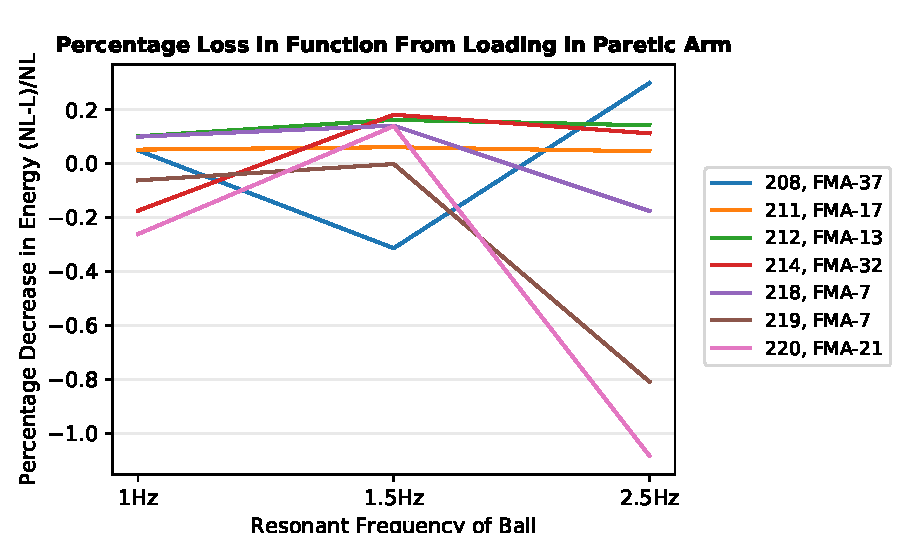
\includegraphics[width=0.49\linewidth]{Plots/pl_A0_indiv_ms.pdf}
     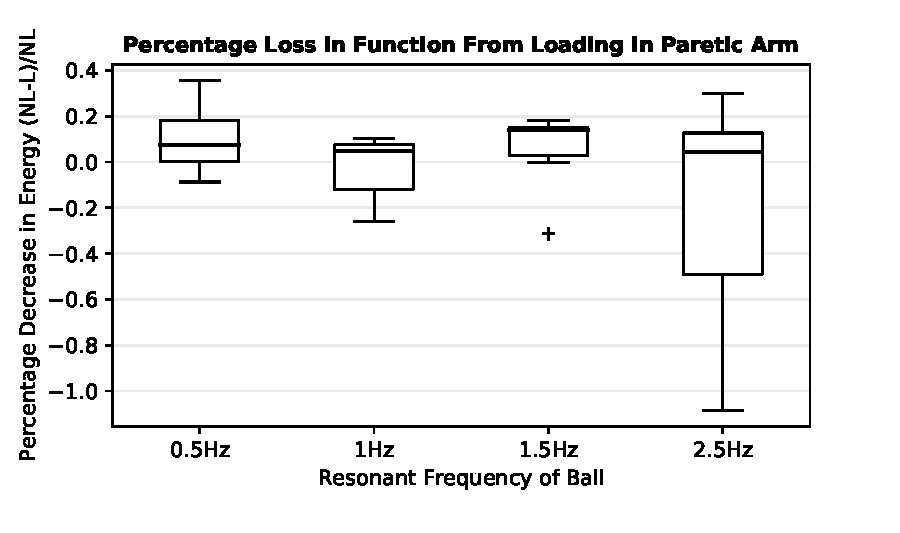
\includegraphics[width=0.49\linewidth]{Plots/pl_A0_ms.pdf}
	\caption{Percent loss in function in the paretic arm due to loading in moderate and severe stroke. Positive values indicate better performance during no loading. Negative values indicate better performance with loading. No trend w.r.t. frequency is apparent (p=0.57). Values are generally positive, indicating better performance without loading. No statistical significance.}
\end{figure}


\begin{figure}[!ht]
     \centering
     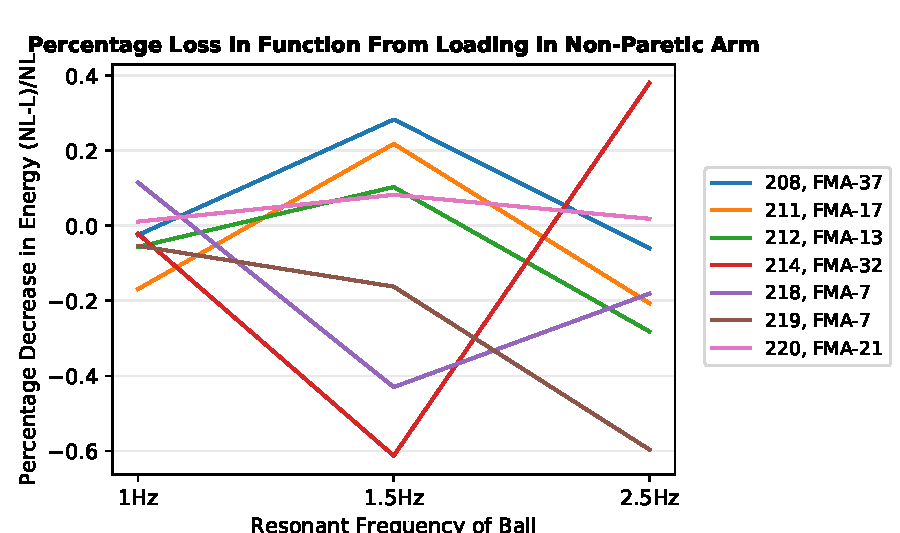
\includegraphics[width=0.49\linewidth]{Plots/pl_A1_indiv_ms.pdf}
     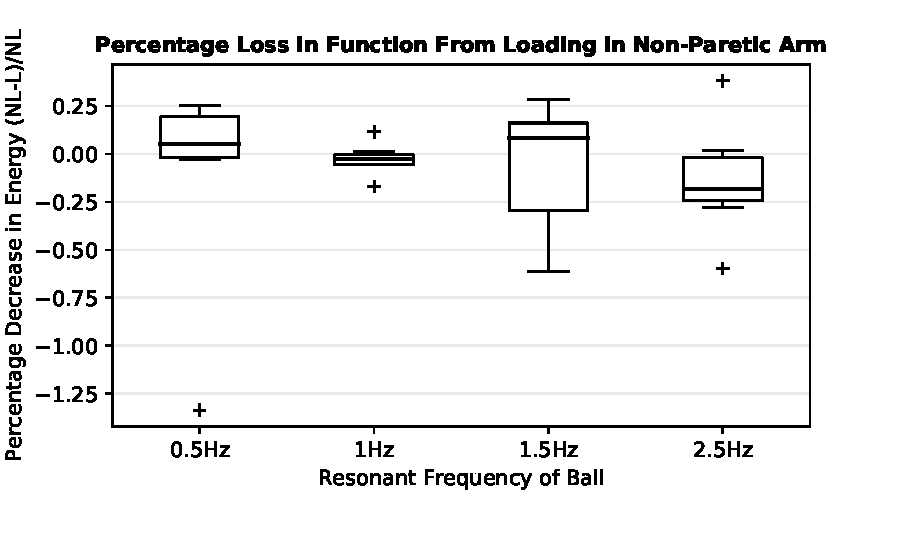
\includegraphics[width=0.49\linewidth]{Plots/pl_A1_ms.pdf}
	\caption{Percent loss in function in the paretic arm due to loading in moderate and severe stroke. Positive values indicate better performance during no loading. Negative values indicate better performance with loading. No trend is apparent.}
\end{figure}


\clearpage
\section{Overall results}

\begin{figure}[!ht]
     \centering
     \subfloat{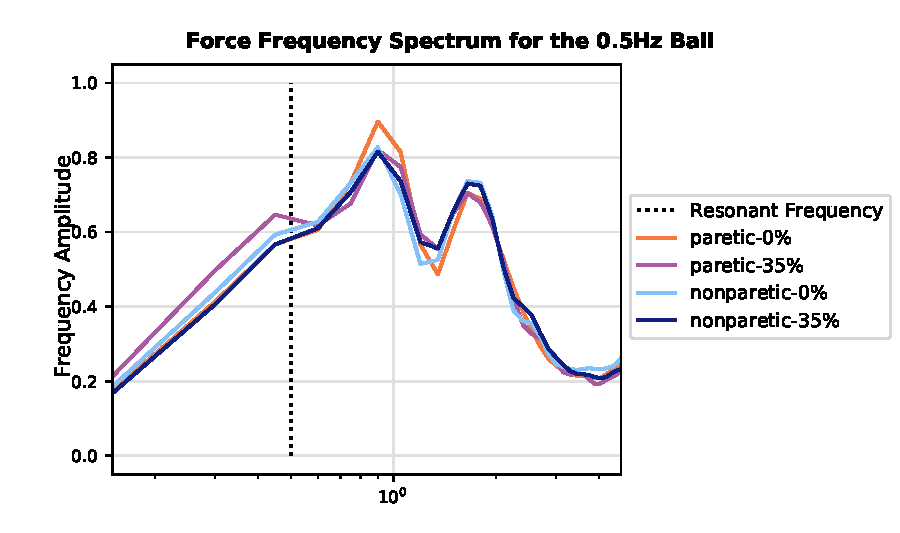
\includegraphics[width=0.49\linewidth]{Plots/agg_spectrum_0.5Hz_all.pdf}}
     \subfloat{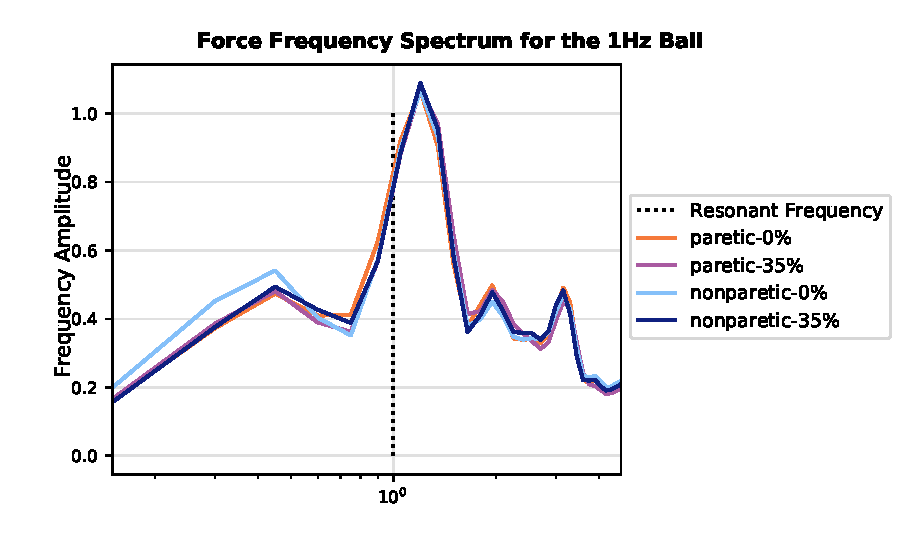
\includegraphics[width=0.49\linewidth]{Plots/agg_spectrum_1Hz_all.pdf}}
     \hfill
     \subfloat{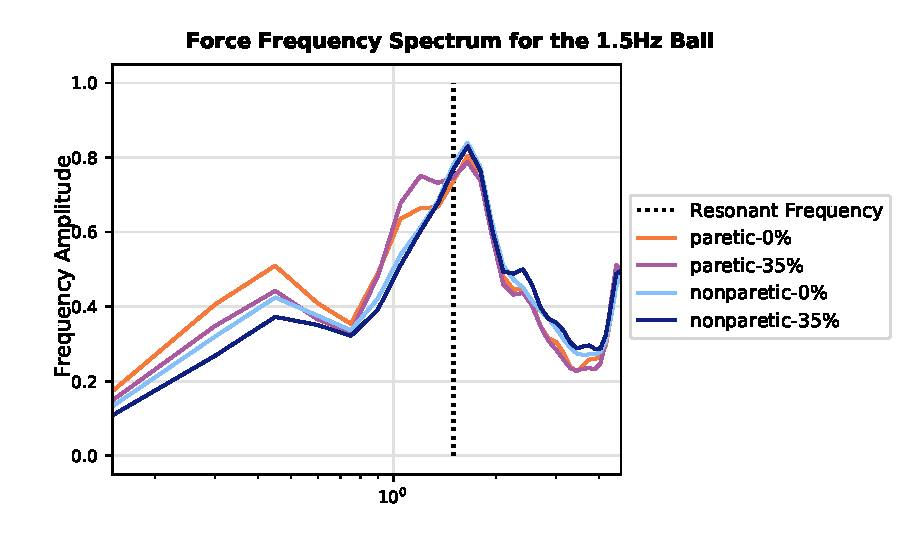
\includegraphics[width=0.49\linewidth]{Plots/agg_spectrum_1.5Hz_all.pdf}}
     \subfloat{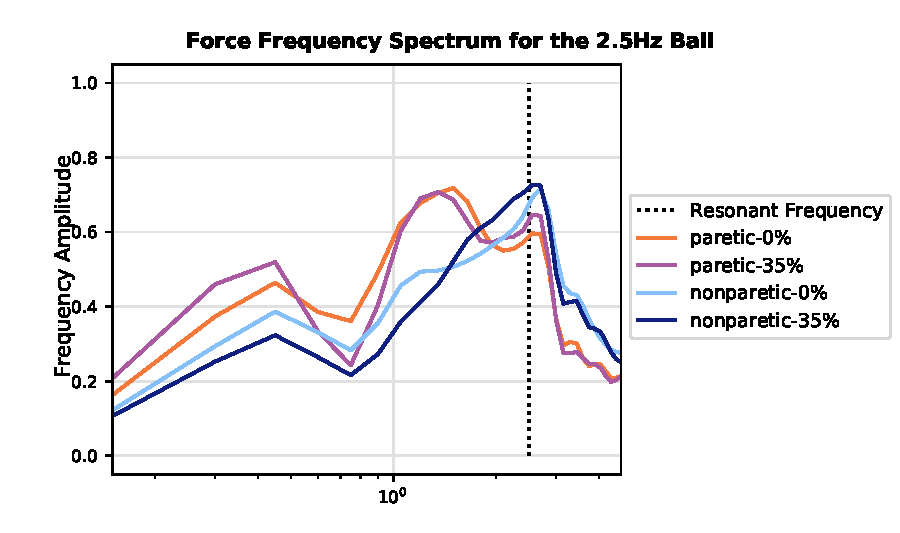
\includegraphics[width=0.49\linewidth]{Plots/agg_spectrum_2.5Hz_all.pdf}}
     \hfill
	\caption{Aggregate Frequency Spectrums. With the 1.5Hz and 2.5Hz ball, participants struggled to reach the resonant frequency with their paretic arm, resulting in a mound (or, for 2.5Hz, a second peak) below the resonant frequency. No trends are apparent at 0.5Hz}
\end{figure}

\begin{figure}[!ht]
     \centering
     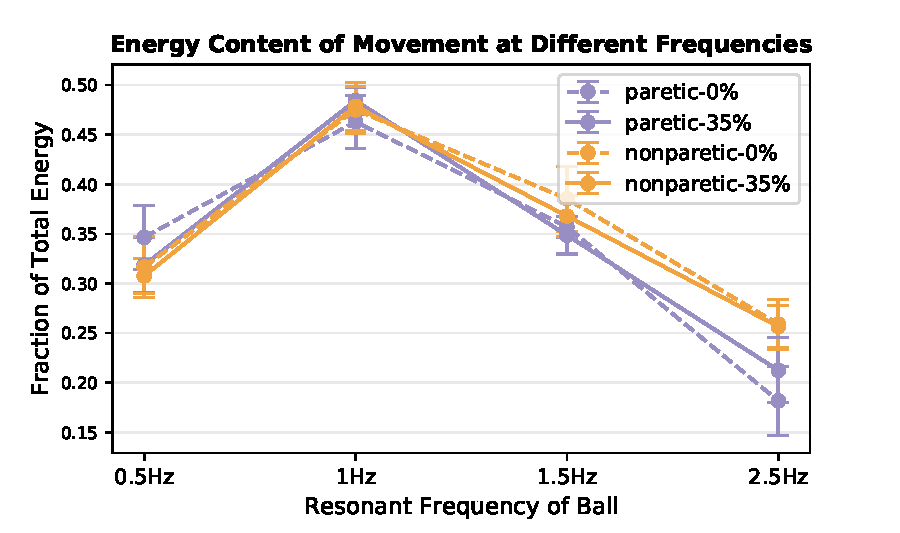
\includegraphics[width=0.49\linewidth]{Plots/e_at_res_raw_all.pdf}
	\caption{Energy at the resonant frequency of the ball metric. No significant factors.}
\end{figure}

\begin{figure}[!ht]
     \centering
     \subfloat{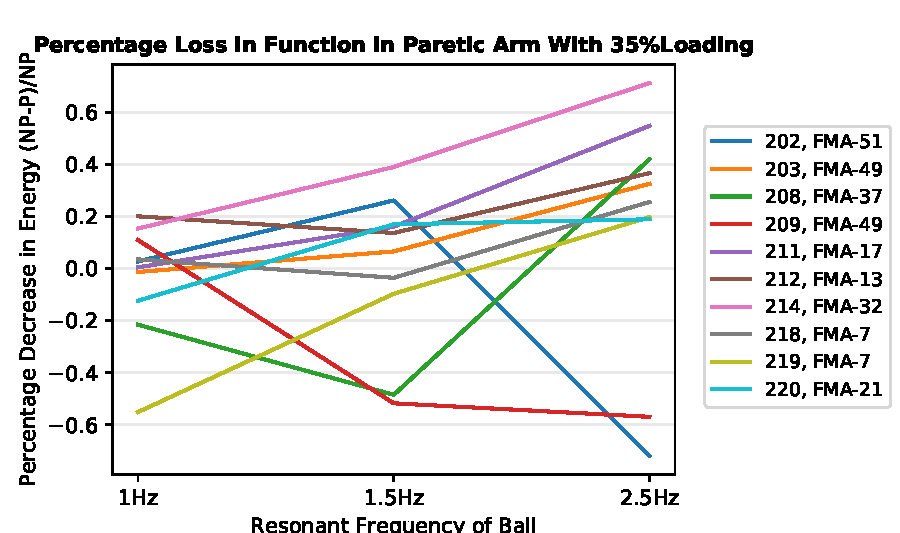
\includegraphics[width=0.49\linewidth]{Plots/pl_SL1_indiv_all.pdf}}
     \subfloat{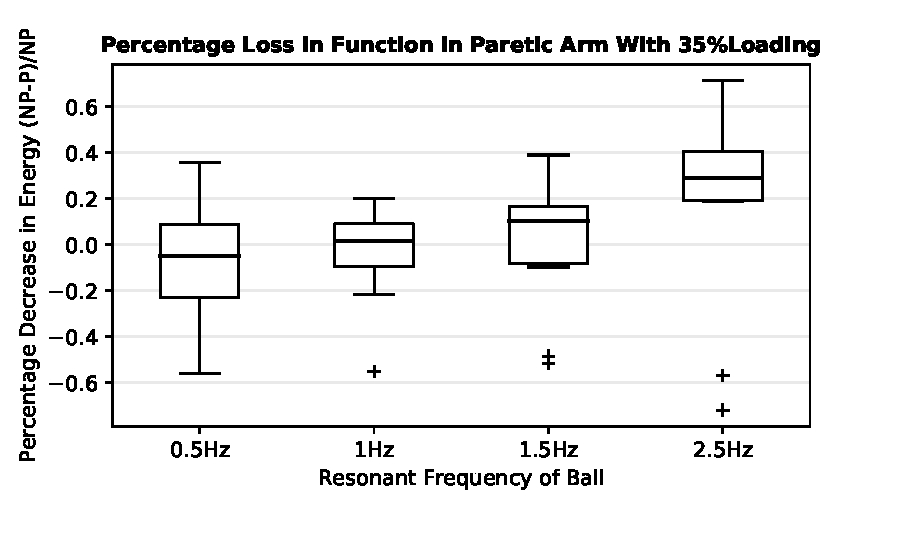
\includegraphics[width=0.49\linewidth]{Plots/pl_SL1_all.pdf}}
     \hfill
	\caption{Percent Decrease in Function in Paretic Arm With Loading. Positive values indicate better performance in the nonparetic arm. Negative values indicate better performance in the paretic arm. }
\end{figure}

\begin{figure}[!ht]
     \centering
     \subfloat{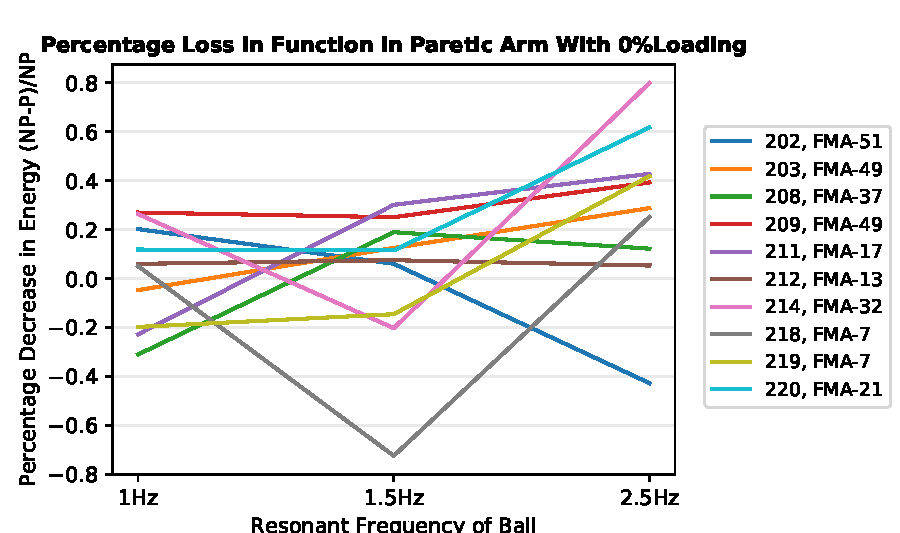
\includegraphics[width=0.49\linewidth]{Plots/pl_SL0_indiv_all.pdf}}
     \subfloat{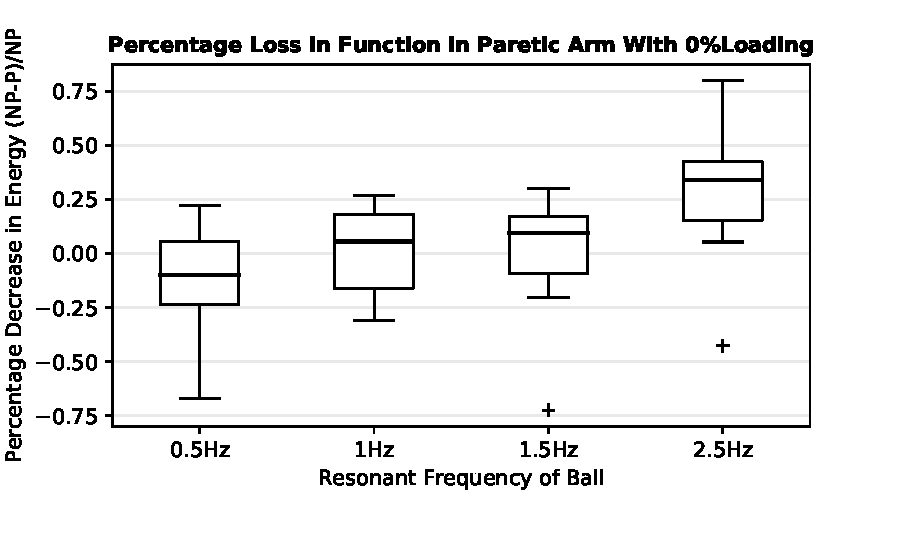
\includegraphics[width=0.49\linewidth]{Plots/pl_SL0_all.pdf}}
     \hfill
	\caption{Percent Decrease in Function in Paretic Arm Without Loading. Positive values indicate better performance in the nonparetic arm. Negative values indicate better performance in the paretic arm.}
\end{figure}


\begin{figure}[!ht]
     \centering
     \subfloat{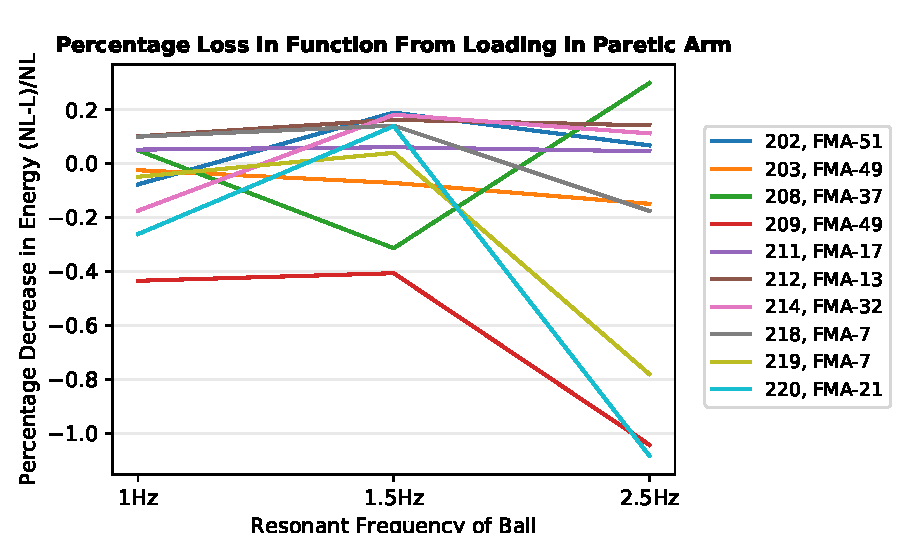
\includegraphics[width=0.49\linewidth]{Plots/pl_A0_indiv_all.pdf}}
     \subfloat{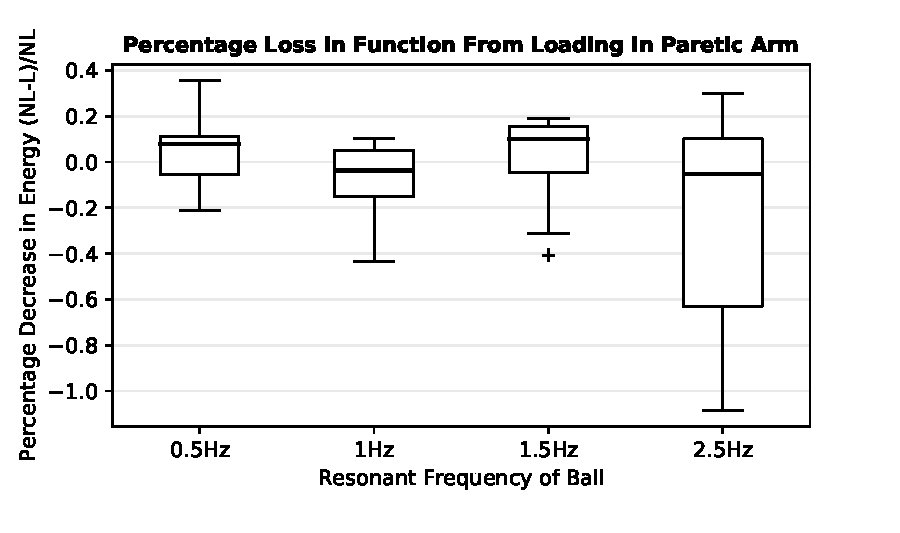
\includegraphics[width=0.49\linewidth]{Plots/pl_A0_all.pdf}}
     \hfill
	\caption{Percent Decrease in Function in Paretic Arm Due to Loading. Positive values indicate better performance during no loading. Negative values indicate better performance with loading.}
\end{figure}


\begin{figure}[!ht]
     \centering
     \subfloat{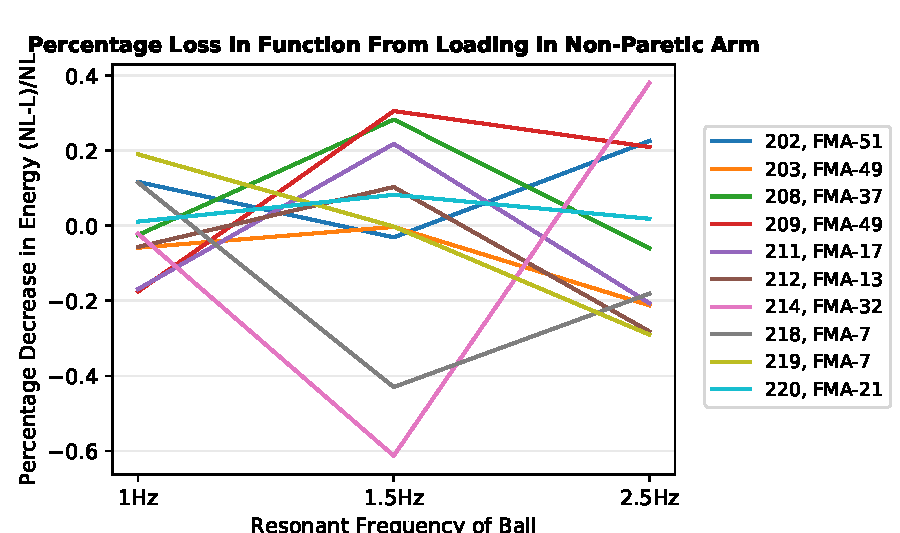
\includegraphics[width=0.49\linewidth]{Plots/pl_A1_indiv_all.pdf}}
     \subfloat{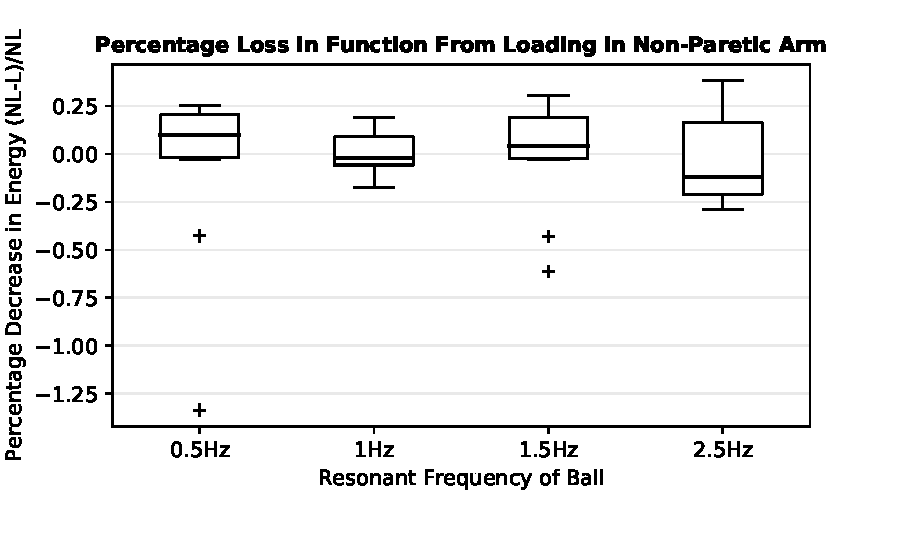
\includegraphics[width=0.49\linewidth]{Plots/pl_A1_all.pdf}}
     \hfill
	\caption{Percent Decrease in Function in Non-Paretic Arm Due to Loading. Positive values indicate better performance during no loading. Negative values indicate better performance with loading. No trend is apparent. }
\end{figure}


\clearpage
\section{Mild Stroke Aggregate Results}

Included participants (N=3): Sub202 (FMA-51), Sub203 (FMA-49), and Sub209 (FMA-49)


\begin{figure}[!ht]
     \centering
     \subfloat{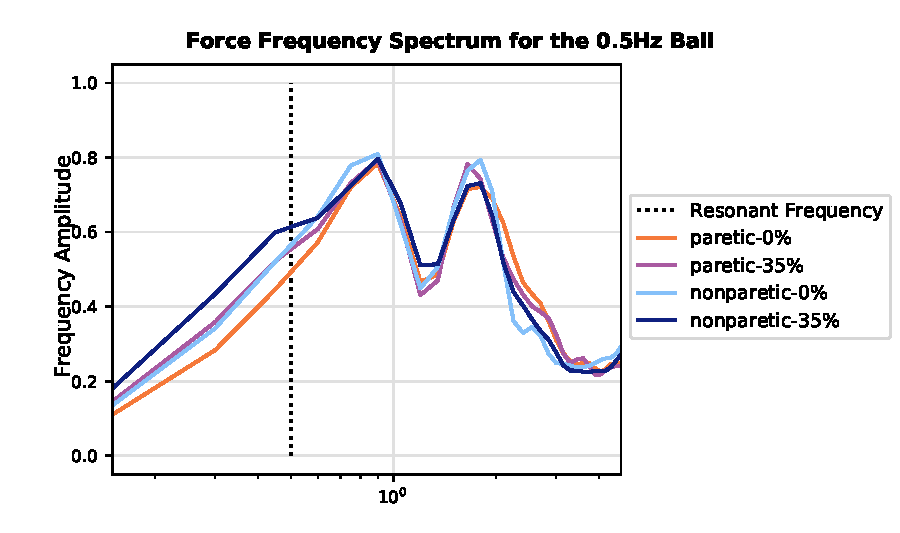
\includegraphics[width=0.49\linewidth]{Plots/agg_spectrum_0.5Hz_m.pdf}}
     \subfloat{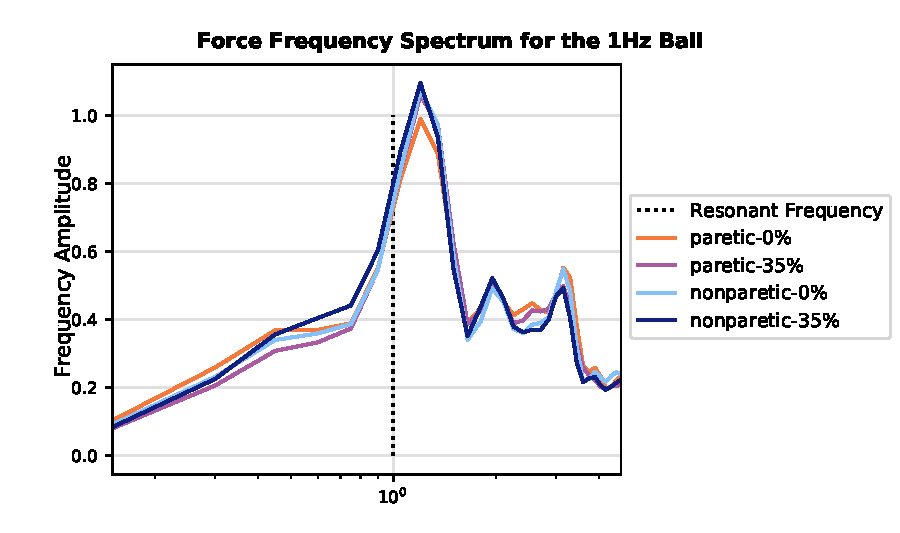
\includegraphics[width=0.49\linewidth]{Plots/agg_spectrum_1Hz_m.pdf}}
     \hfill
     \subfloat{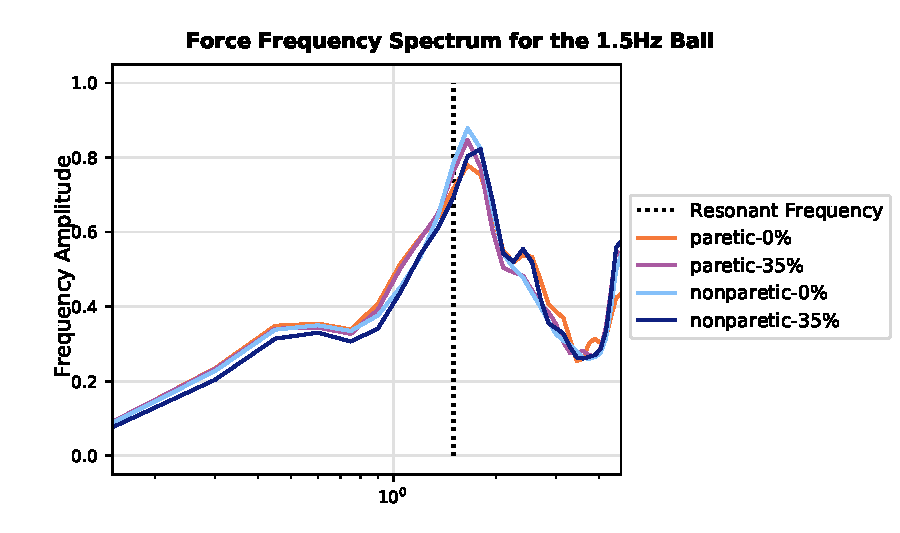
\includegraphics[width=0.49\linewidth]{Plots/agg_spectrum_1.5Hz_m.pdf}}
     \subfloat{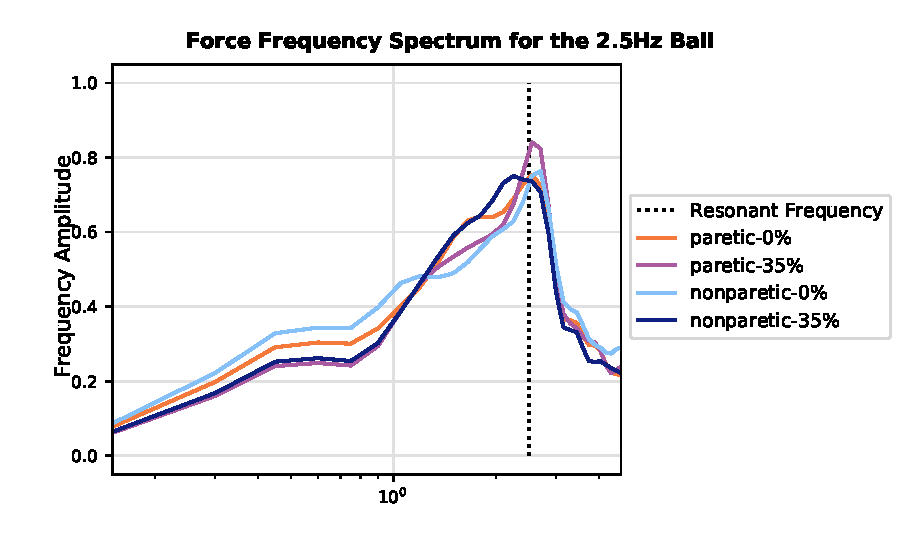
\includegraphics[width=0.49\linewidth]{Plots/agg_spectrum_2.5Hz_m.pdf}}
     \hfill
	\caption{Aggregate Frequency Spectrums for participants with mild stroke.}
\end{figure}

\begin{figure}[!ht]
     \centering
     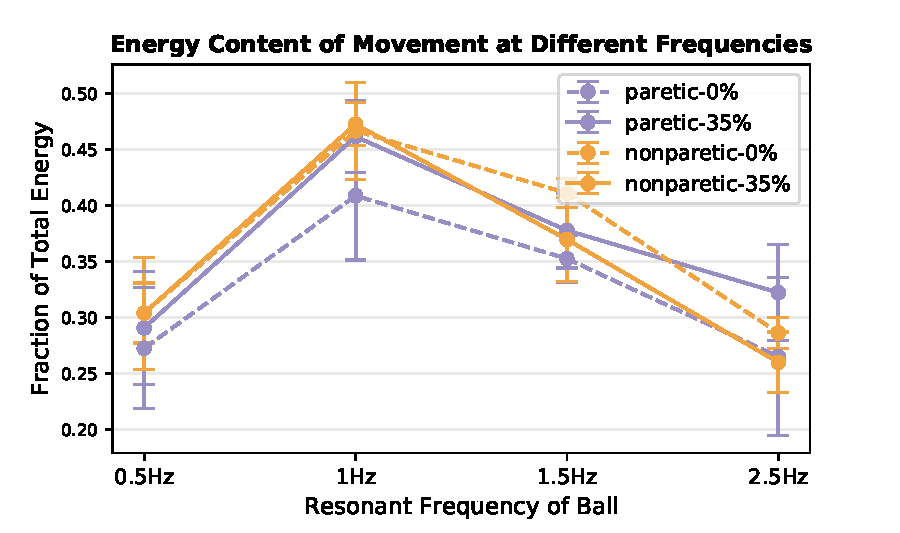
\includegraphics[width=0.49\linewidth]{Plots/e_at_res_raw_m.pdf}
	\caption{Energy at the resonant frequency of the ball metric for participants with moderate and severe stroke.}
\end{figure}

\begin{figure}[!ht]
     \centering
     \subfloat{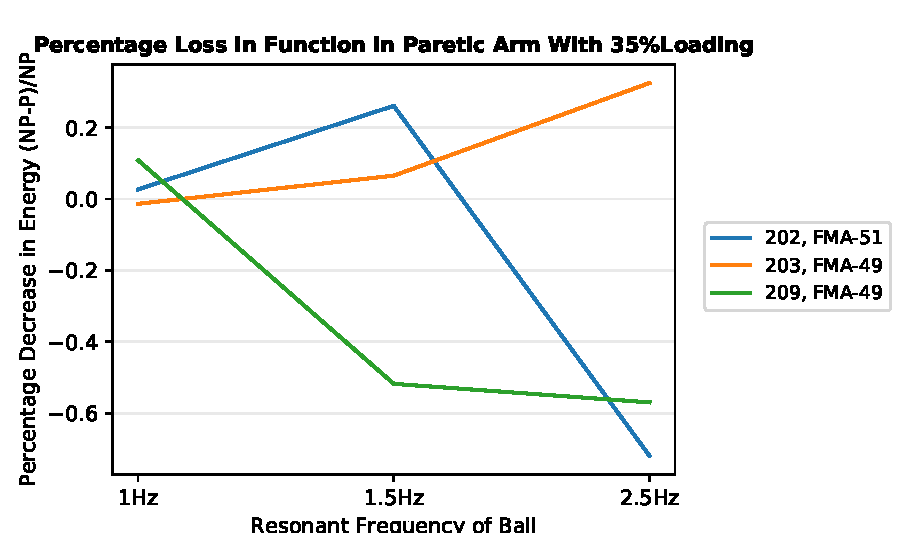
\includegraphics[width=0.49\linewidth]{Plots/pl_SL1_indiv_m.pdf}}
     \subfloat{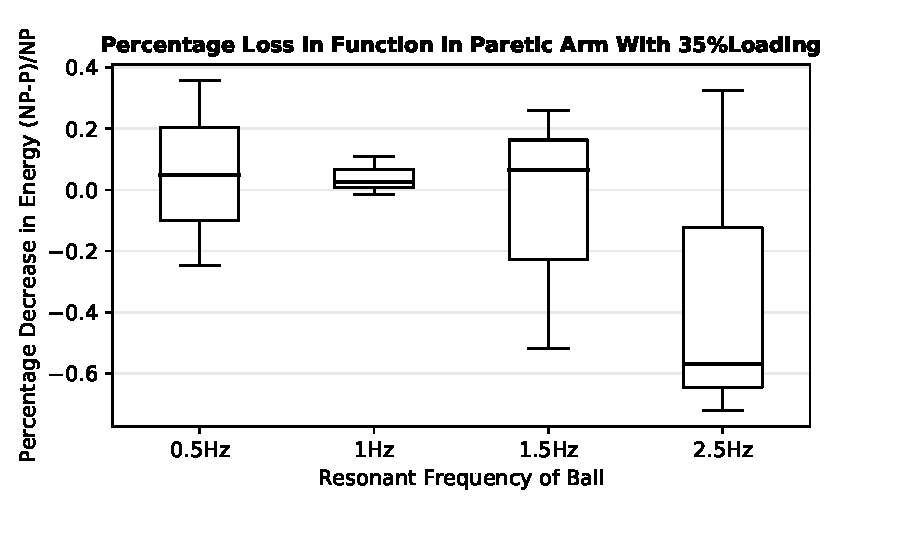
\includegraphics[width=0.49\linewidth]{Plots/pl_SL1_m.pdf}}
     \hfill
	\caption{Percent Decrease in Function in Paretic Arm With Loading. Positive values indicate better performance in the nonparetic arm. Negative values indicate better performance in the paretic arm. }
\end{figure}

\begin{figure}[!ht]
     \centering
     \subfloat{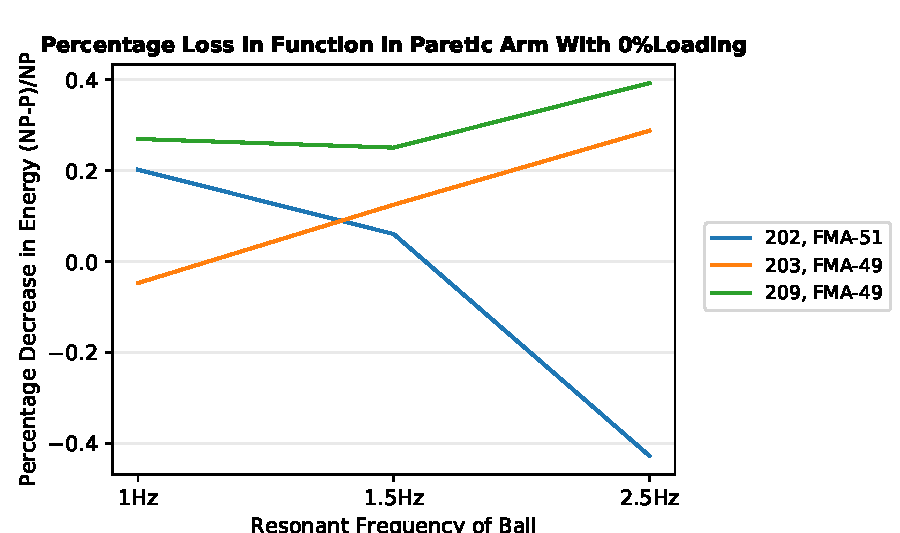
\includegraphics[width=0.49\linewidth]{Plots/pl_SL0_indiv_m.pdf}}
     \subfloat{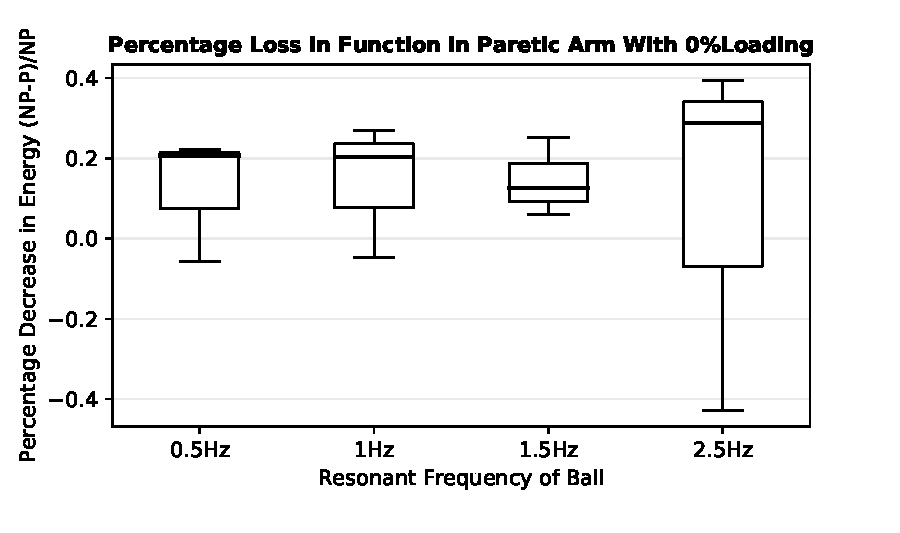
\includegraphics[width=0.49\linewidth]{Plots/pl_SL0_m.pdf}}
     \hfill
	\caption{Percent Decrease in Function in Paretic Arm Without Loading. Positive values indicate better performance in the nonparetic arm. Negative values indicate better performance in the paretic arm. }
\end{figure}


\begin{figure}[!ht]
     \centering
     \subfloat{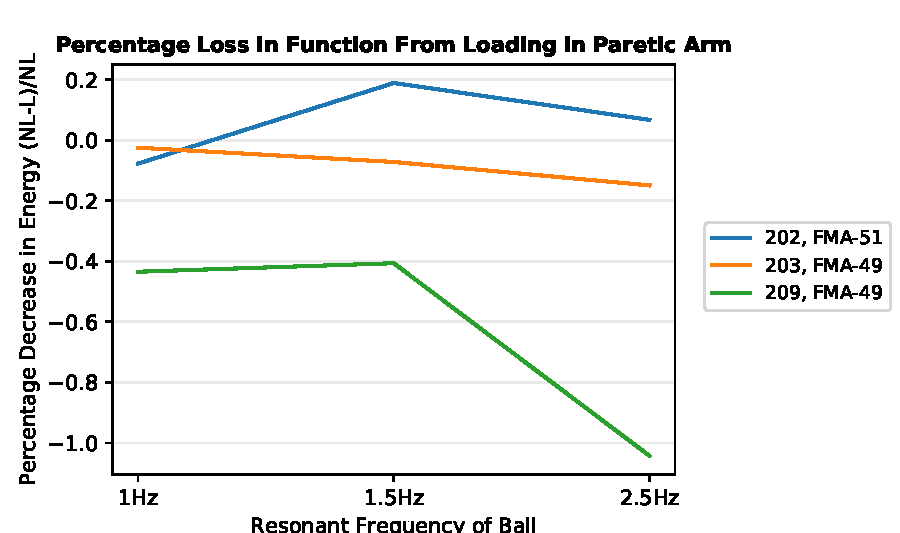
\includegraphics[width=0.49\linewidth]{Plots/pl_A0_indiv_m.pdf}}
     \subfloat{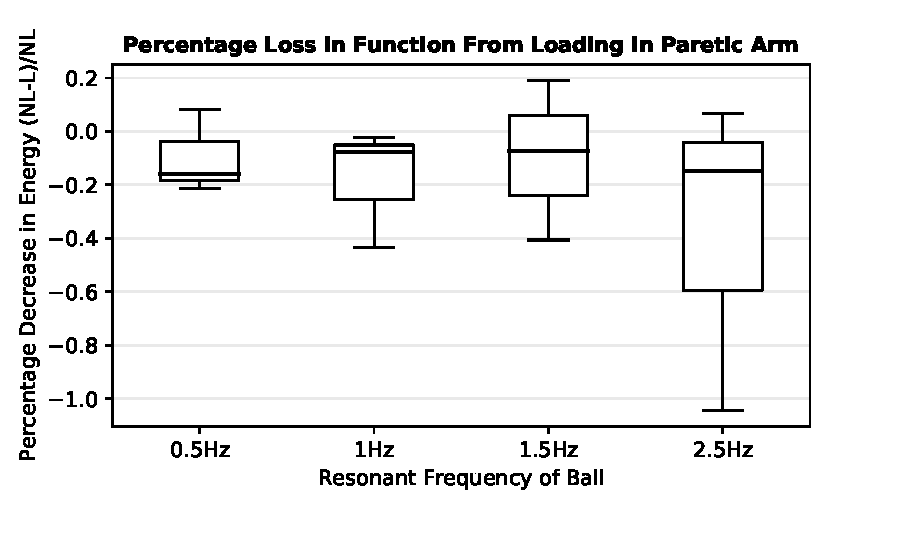
\includegraphics[width=0.49\linewidth]{Plots/pl_A0_m.pdf}}
     \hfill
	\caption{Percent Decrease in Function in Paretic Arm Due to Loading. Positive values indicate better performance during no loading. Negative values indicate better performance with loading.}
\end{figure}


\begin{figure}[!ht]
     \centering
     \subfloat{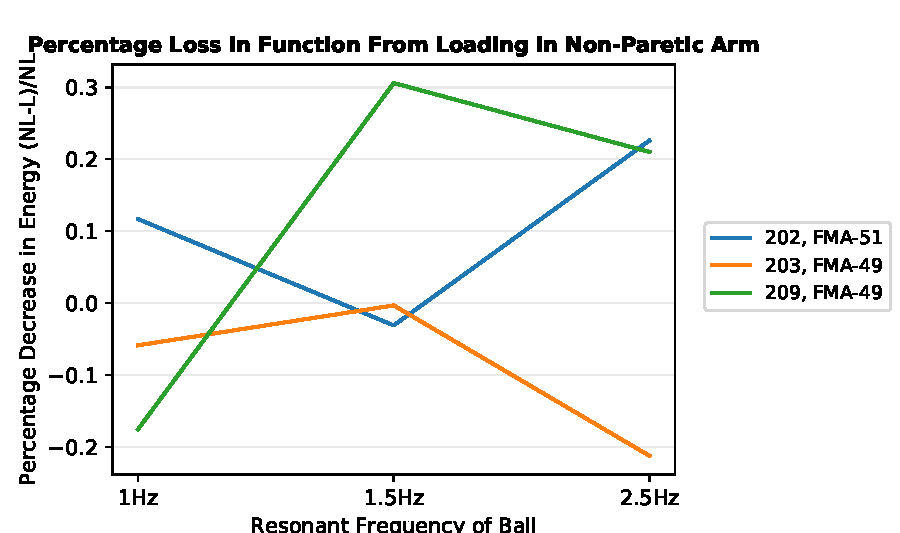
\includegraphics[width=0.49\linewidth]{Plots/pl_A1_indiv_m.pdf}}
     \subfloat{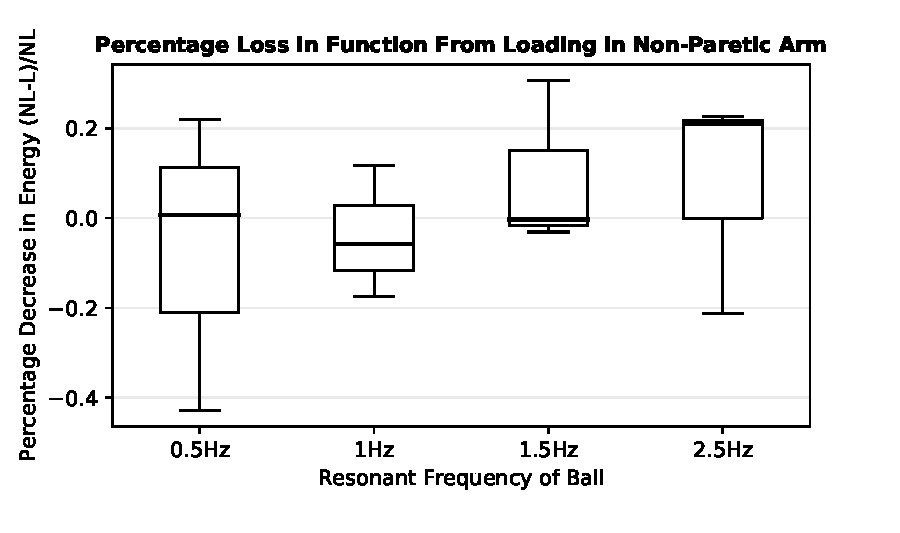
\includegraphics[width=0.49\linewidth]{Plots/pl_A1_m.pdf}}
     \hfill
	\caption{Percent Decrease in Function in Non-Paretic Arm Due to Loading. Positive values indicate better performance during no loading. Negative values indicate better performance with loading.}
\end{figure}

\clearpage
\section{Individual Subject Results}

\subsection{S202; FMA = 51}

\begin{figure}[!ht]
     \centering
     \subfloat{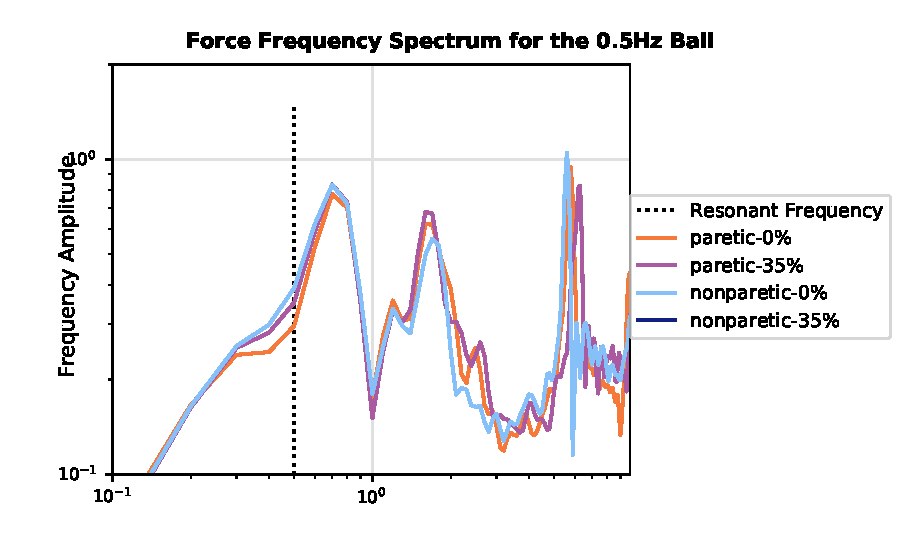
\includegraphics[width=0.49\linewidth]{Plots/IndividualSubjectPlots/S202/S202_0.5Hz.pdf}}
     \subfloat{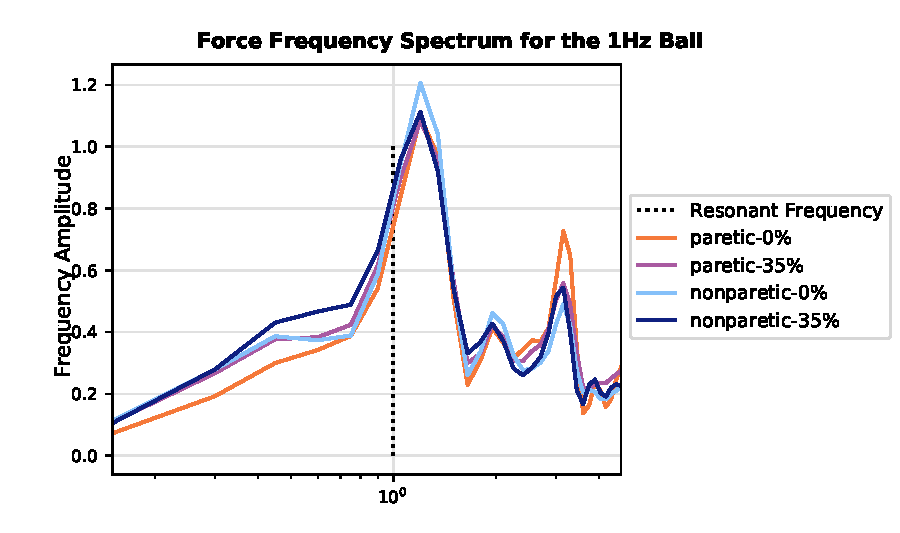
\includegraphics[width=0.49\linewidth]{Plots/IndividualSubjectPlots/S202/S202_1Hz.pdf}}
     \hfill
     \subfloat{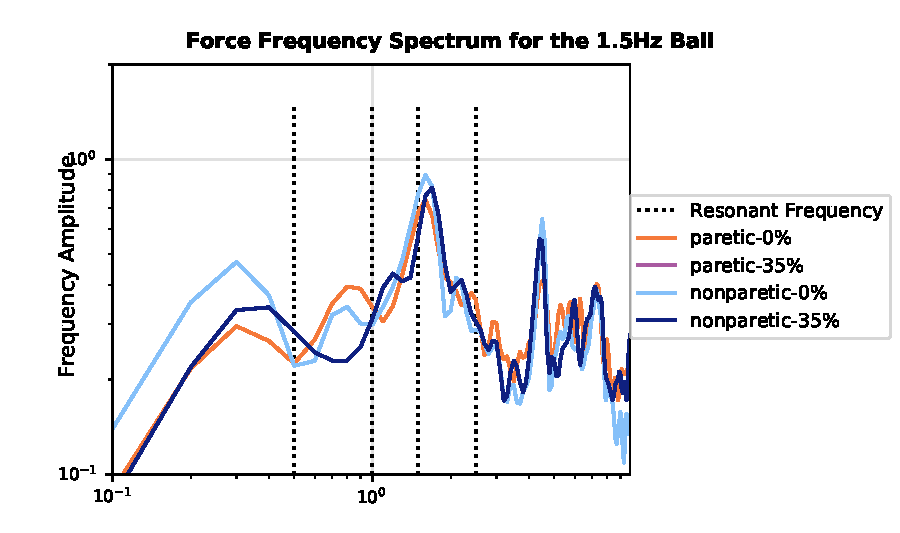
\includegraphics[width=0.49\linewidth]{Plots/IndividualSubjectPlots/S202/S202_1.5Hz.pdf}}
     \subfloat{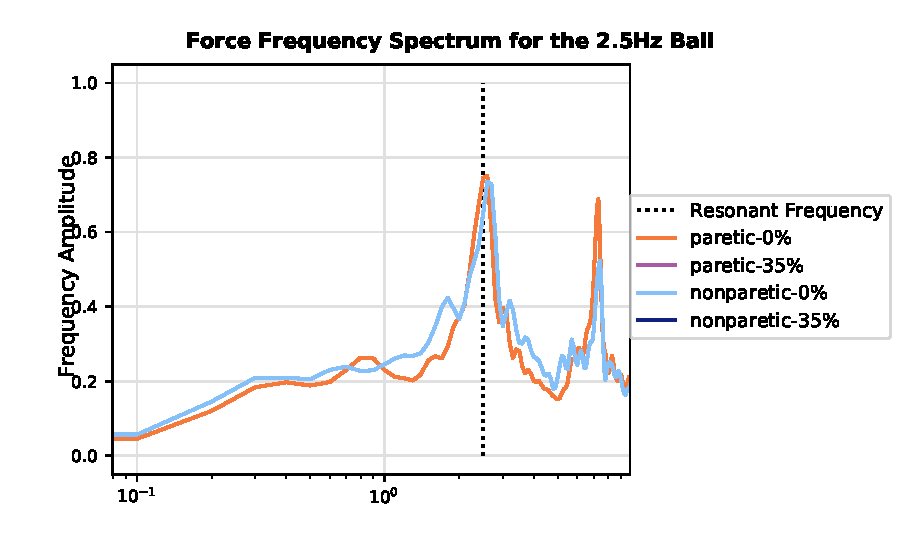
\includegraphics[width=0.49\linewidth]{Plots/IndividualSubjectPlots/S202/S202_2.5Hz.pdf}}
     \hfill
     \subfloat{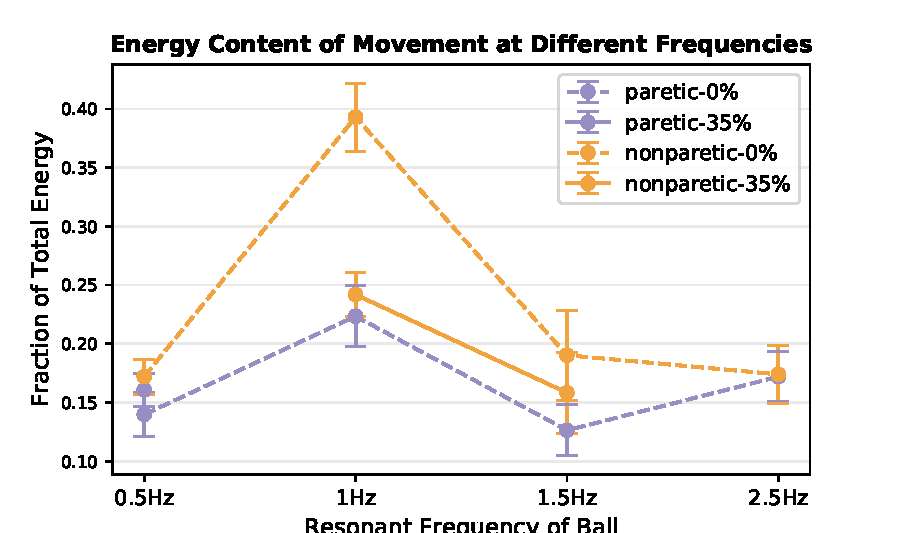
\includegraphics[width=0.49\linewidth]{Plots/IndividualSubjectPlots/S202/S202.pdf}}
	\caption{Subject 202 Frequency Spectrums. Interation effect between arm and ball frequency (p$<$0.001). Arm is a significant factor for 2.5Hz (p=0.001).}
\end{figure}

\clearpage
\subsection{S203; FMA = 49}

\begin{figure}[!ht]
     \centering
     \subfloat{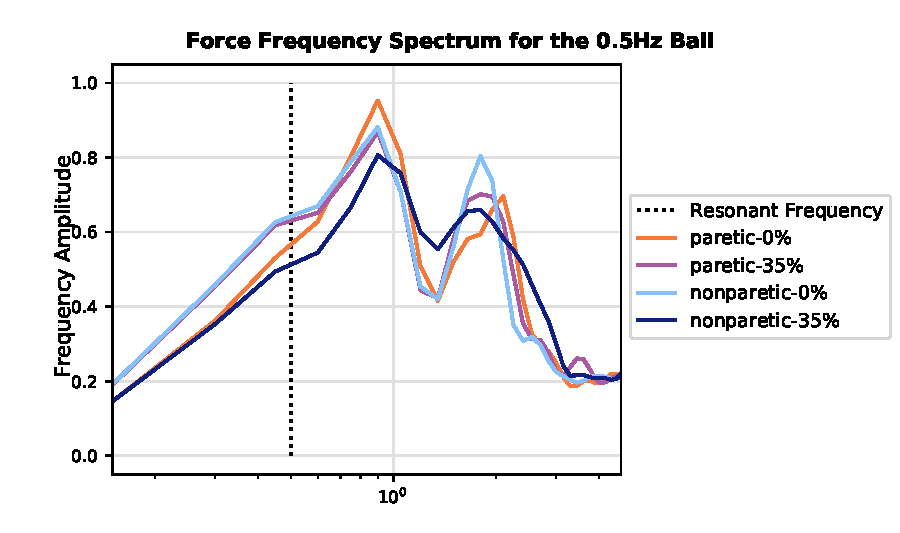
\includegraphics[width=0.49\linewidth]{Plots/IndividualSubjectPlots/S203/S203_0.5Hz.pdf}}
     \subfloat{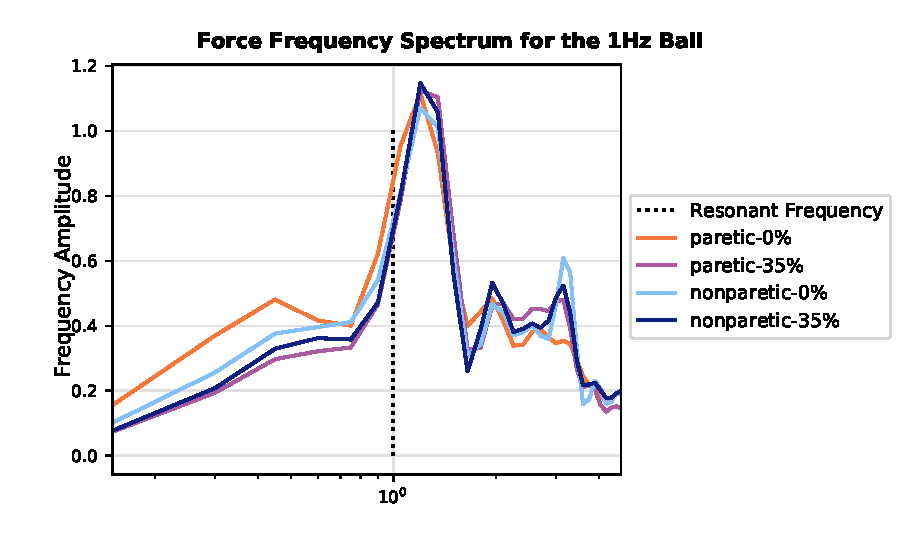
\includegraphics[width=0.49\linewidth]{Plots/IndividualSubjectPlots/S203/S203_1Hz.pdf}}
     \hfill
     \subfloat{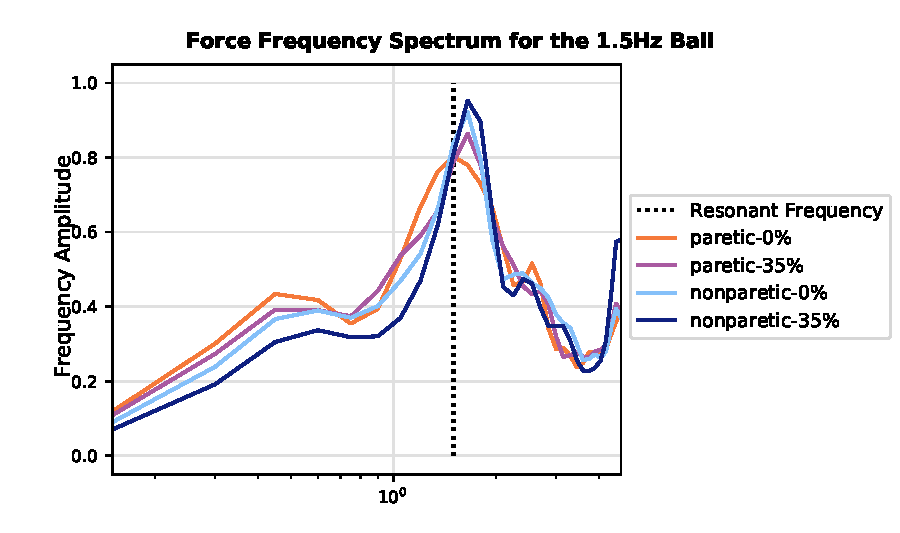
\includegraphics[width=0.49\linewidth]{Plots/IndividualSubjectPlots/S203/S203_1.5Hz.pdf}}
     \subfloat{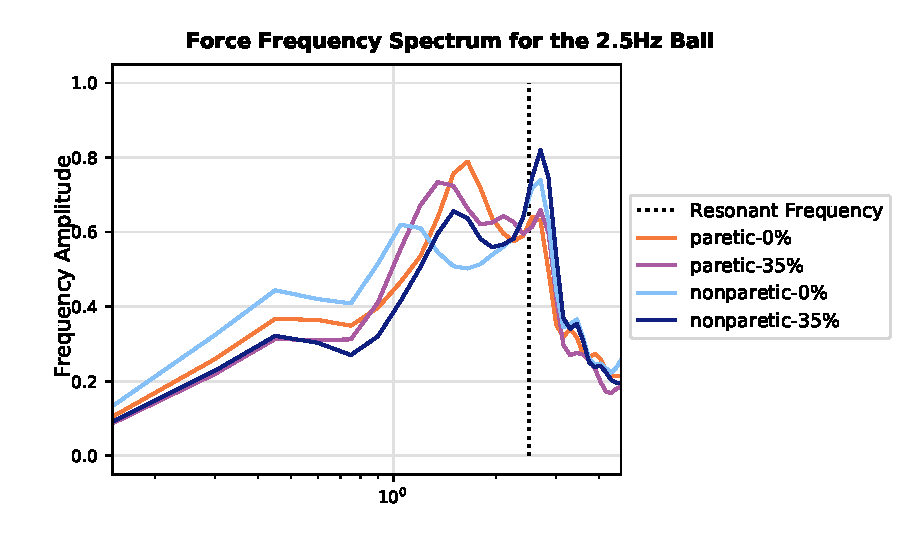
\includegraphics[width=0.49\linewidth]{Plots/IndividualSubjectPlots/S203/S203_2.5Hz.pdf}}
     \hfill
     \subfloat{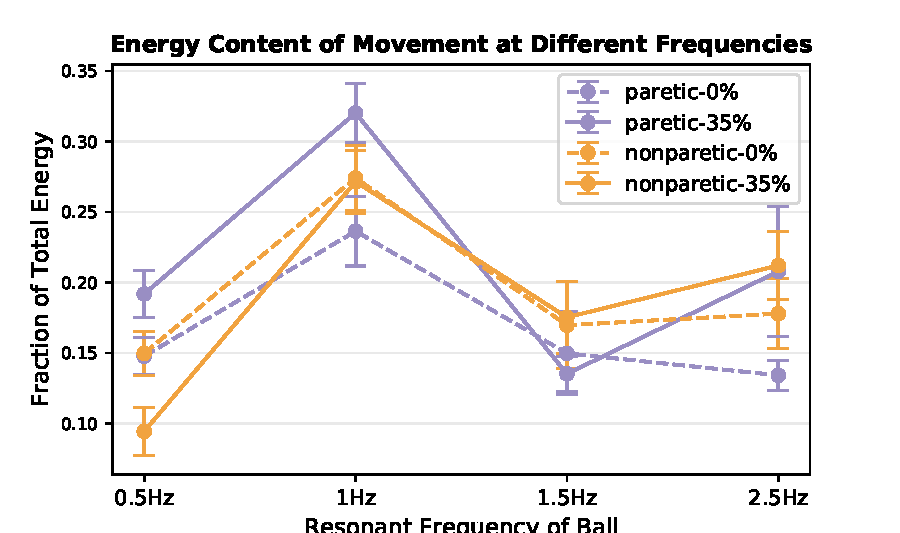
\includegraphics[width=0.49\linewidth]{Plots/IndividualSubjectPlots/S203/S203.pdf}}
	\caption{Subject 203 Frequency Spectrums. Interation effect between arm and ball frequency (p=0.013). For the 2.5Hz ball, arm is a significant factor (p=0.037).}
\end{figure}

\clearpage
\subsection{S205; FMA = 34}

The participant was not able to match the resonant frequency of the 1.5Hz and 2.5Hz balls with their nonparetic limb. Therefore, this participant was removed from the aggregate analyses.

\begin{figure}[!ht]
     \centering
     \subfloat{\includegraphics[width=0.49\linewidth]{Plots/IndividualSubjectPlots/S205/S205_0.5Hz.pdf}}
     \subfloat{\includegraphics[width=0.49\linewidth]{Plots/IndividualSubjectPlots/S205/S205_1Hz.pdf}}
     \hfill
     \subfloat{\includegraphics[width=0.49\linewidth]{Plots/IndividualSubjectPlots/S205/S205_1.5Hz.pdf}}
     \subfloat{\includegraphics[width=0.49\linewidth]{Plots/IndividualSubjectPlots/S205/S205_2.5Hz.pdf}}
     \hfill
     \subfloat{\includegraphics[width=0.49\linewidth]{Plots/IndividualSubjectPlots/S205/S205.pdf}}
	\caption{Subject 205 Frequency Spectrums}
\end{figure}

\clearpage
\subsection{S207; FMA = 30}

The participant was not able to match the resonant frequency of the 1.5Hz and 2.5Hz balls with their nonparetic limb. Therefore, this participant was removed from the aggregate analyses.

\begin{figure}[!ht]
     \centering
     \subfloat{\includegraphics[width=0.49\linewidth]{Plots/IndividualSubjectPlots/S207/S207_0.5Hz.pdf}}
     \subfloat{\includegraphics[width=0.49\linewidth]{Plots/IndividualSubjectPlots/S207/S207_1Hz.pdf}}
     \hfill
     \subfloat{\includegraphics[width=0.49\linewidth]{Plots/IndividualSubjectPlots/S207/S207_1.5Hz.pdf}}
     \subfloat{\includegraphics[width=0.49\linewidth]{Plots/IndividualSubjectPlots/S207/S207_2.5Hz.pdf}}
     \hfill
     \subfloat{\includegraphics[width=0.49\linewidth]{Plots/IndividualSubjectPlots/S207/S207.pdf}}
	\caption{Subject 207 Frequency Spectrums}
\end{figure}

\clearpage
\subsection{S208; FMA = 37}

\begin{figure}[!ht]
     \centering
     \subfloat{\includegraphics[width=0.49\linewidth]{Plots/IndividualSubjectPlots/S208/S208_0.5Hz.pdf}}
     \subfloat{\includegraphics[width=0.49\linewidth]{Plots/IndividualSubjectPlots/S208/S208_1Hz.pdf}}
     \hfill
     \subfloat{\includegraphics[width=0.49\linewidth]{Plots/IndividualSubjectPlots/S208/S208_1.5Hz.pdf}}
     \subfloat{\includegraphics[width=0.49\linewidth]{Plots/IndividualSubjectPlots/S208/S208_2.5Hz.pdf}}
     \hfill
     \subfloat{\includegraphics[width=0.49\linewidth]{Plots/IndividualSubjectPlots/S208/S208.pdf}}
	\caption{Subject 208 Frequency Spectrums. Interation effect between arm and ball frequency (p=0.0007). For the 1Hz and 2.5Hz ball, arm is a significant factor, p=0.001 and p=0.021 respectively. There is an interaction effect between ball frequency and loading in the paretic arm (p=0.022).}
\end{figure}

\clearpage
\subsection{S209; FMA = 49}

\begin{figure}[!ht]
     \centering
     \subfloat{\includegraphics[width=0.49\linewidth]{Plots/IndividualSubjectPlots/S209/S209_0.5Hz.pdf}}
     \subfloat{\includegraphics[width=0.49\linewidth]{Plots/IndividualSubjectPlots/S209/S209_1Hz.pdf}}
     \hfill
     \subfloat{\includegraphics[width=0.49\linewidth]{Plots/IndividualSubjectPlots/S209/S209_1.5Hz.pdf}}
     \subfloat{\includegraphics[width=0.49\linewidth]{Plots/IndividualSubjectPlots/S209/S209_2.5Hz.pdf}}
     \hfill
     \subfloat{\includegraphics[width=0.49\linewidth]{Plots/IndividualSubjectPlots/S209/S209.pdf}}
	\caption{Subject 209 Frequency Spectrums. Interation effect between arm and ball frequency (p=0.0003) and pretty much everything is significant}%Loading is significant (p=0.002). Interaction effect between arm, ball frequency, and loading (p=0.002). At 1Hz, arm (p=0.046) is significant; Loading (p=0.011) is significant together and in both arms individually. At 1.5Hz and 2.5Hz, there is an interaction effect between loading and arm and there is a strong loading trends in each arms individually. Loading is a significant fatcor in the paretic arm (p=2.93E-5). In the non-paretic arm, there is an interaction effect between ball frequency and loading.}
\end{figure}


\clearpage
\subsection{S211; FMA = 17}

\begin{figure}[!ht]
     \centering
     \subfloat{\includegraphics[width=0.49\linewidth]{Plots/IndividualSubjectPlots/S211/S211_0.5Hz.pdf}}
     \subfloat{\includegraphics[width=0.49\linewidth]{Plots/IndividualSubjectPlots/S211/S211_1Hz.pdf}}
     \hfill
     \subfloat{\includegraphics[width=0.49\linewidth]{Plots/IndividualSubjectPlots/S211/S211_1.5Hz.pdf}}
     \subfloat{\includegraphics[width=0.49\linewidth]{Plots/IndividualSubjectPlots/S211/S211_2.5Hz.pdf}}
     \hfill
     \subfloat{\includegraphics[width=0.49\linewidth]{Plots/IndividualSubjectPlots/S211/S211.pdf}}
	\caption{Subject 211 Frequency Spectrums. Interation effect between arm and ball frequency. Arm is a significant factor overall and for 1.5Hz and 2.5Hz.}
\end{figure}

\clearpage
\subsection{S212; FMA = 13}

\begin{figure}[!ht]
     \centering
     \subfloat{\includegraphics[width=0.49\linewidth]{Plots/IndividualSubjectPlots/S212/S212_0.5Hz.pdf}}
     \subfloat{\includegraphics[width=0.49\linewidth]{Plots/IndividualSubjectPlots/S212/S212_1Hz.pdf}}
     \hfill
     \subfloat{\includegraphics[width=0.49\linewidth]{Plots/IndividualSubjectPlots/S212/S212_1.5Hz.pdf}}
     \subfloat{\includegraphics[width=0.49\linewidth]{Plots/IndividualSubjectPlots/S212/S212_2.5Hz.pdf}}
     \hfill
     \subfloat{\includegraphics[width=0.49\linewidth]{Plots/IndividualSubjectPlots/S212/S212.pdf}}
	\caption{Subject 212 Frequency Spectrums. Interation effect between arm and ball frequency (p<0.0001).}
\end{figure}

\clearpage
\subsection{S214; FMA = 32}

\begin{figure}[!ht]
     \centering
     \subfloat{\includegraphics[width=0.49\linewidth]{Plots/IndividualSubjectPlots/S214/S214_0.5Hz.pdf}}
     \subfloat{\includegraphics[width=0.49\linewidth]{Plots/IndividualSubjectPlots/S214/S214_1Hz.pdf}}
     \hfill
     \subfloat{\includegraphics[width=0.49\linewidth]{Plots/IndividualSubjectPlots/S214/S214_1.5Hz.pdf}}
     \subfloat{\includegraphics[width=0.49\linewidth]{Plots/IndividualSubjectPlots/S214/S214_2.5Hz.pdf}}
     \hfill
     \subfloat{\includegraphics[width=0.49\linewidth]{Plots/IndividualSubjectPlots/S214/S214.pdf}}
	\caption{Subject 214 Frequency Spectrums. Interation effect between arm and ball frequency (p<0.0001). Arm is significant factor. Interaction effect between ball frequency and loading. Arm is significant at 1Hz and 2.5Hz. }
\end{figure}

\clearpage
\subsection{S215; FMA =}

The participant was not able to match the resonant frequency of the 1.5Hz and 2.5Hz balls with their nonparetic limb. Therefore, this participant was removed from the aggregate analyses.

\begin{figure}[!ht]
     \centering
     \subfloat{\includegraphics[width=0.49\linewidth]{Plots/IndividualSubjectPlots/S215/S215_0.5Hz.pdf}}
     \subfloat{\includegraphics[width=0.49\linewidth]{Plots/IndividualSubjectPlots/S215/S215_1Hz.pdf}}
     \hfill
     \subfloat{\includegraphics[width=0.49\linewidth]{Plots/IndividualSubjectPlots/S215/S215_1.5Hz.pdf}}
     \subfloat{\includegraphics[width=0.49\linewidth]{Plots/IndividualSubjectPlots/S215/S215_2.5Hz.pdf}}
     \hfill
     \subfloat{\includegraphics[width=0.49\linewidth]{Plots/IndividualSubjectPlots/S215/S215.pdf}}
	\caption{Subject 215 Frequency Spectrums.}
\end{figure}

\clearpage
\subsection{S216; FMA =}

The participant was not able to match the resonant frequency of the 2.5Hz ball with their nonparetic limb. Therefore, this participant was removed from the aggregate analyses.

\begin{figure}[!ht]
     \centering
     \subfloat{\includegraphics[width=0.49\linewidth]{Plots/IndividualSubjectPlots/S216/S216_0.5Hz.pdf}}
     \subfloat{\includegraphics[width=0.49\linewidth]{Plots/IndividualSubjectPlots/S216/S216_1Hz.pdf}}
     \hfill
     \subfloat{\includegraphics[width=0.49\linewidth]{Plots/IndividualSubjectPlots/S216/S216_1.5Hz.pdf}}
     \subfloat{\includegraphics[width=0.49\linewidth]{Plots/IndividualSubjectPlots/S216/S216_2.5Hz.pdf}}
     \hfill
     \subfloat{\includegraphics[width=0.49\linewidth]{Plots/IndividualSubjectPlots/S216/S216.pdf}}
	\caption{Subject 216 Frequency Spectrums.}
\end{figure}

\clearpage
\subsection{S217; FMA =}

The participant was not able to match the resonant frequency of the 2.5Hz ball with their nonparetic limb. Additionally, the participant's abduction strength is zero. Therefore, this participant was removed from the aggregate analyses.

\begin{figure}[!ht]
     \centering
     \subfloat{\includegraphics[width=0.49\linewidth]{Plots/IndividualSubjectPlots/S217/S217_0.5Hz.pdf}}
     \subfloat{\includegraphics[width=0.49\linewidth]{Plots/IndividualSubjectPlots/S217/S217_1Hz.pdf}}
     \hfill
     \subfloat{\includegraphics[width=0.49\linewidth]{Plots/IndividualSubjectPlots/S217/S217_1.5Hz.pdf}}
     \subfloat{\includegraphics[width=0.49\linewidth]{Plots/IndividualSubjectPlots/S217/S217_2.5Hz.pdf}}
     \hfill
     \subfloat{\includegraphics[width=0.49\linewidth]{Plots/IndividualSubjectPlots/S217/S217.pdf}}
	\caption{Subject 217 Frequency Spectrums.}
\end{figure}

\clearpage
\subsection{S218; FMA = 7}

\begin{figure}[!ht]
     \centering
     \subfloat{\includegraphics[width=0.49\linewidth]{Plots/IndividualSubjectPlots/S218/S218_0.5Hz.pdf}}
     \subfloat{\includegraphics[width=0.49\linewidth]{Plots/IndividualSubjectPlots/S218/S218_1Hz.pdf}}
     \hfill
     \subfloat{\includegraphics[width=0.49\linewidth]{Plots/IndividualSubjectPlots/S218/S218_1.5Hz.pdf}}
     \subfloat{\includegraphics[width=0.49\linewidth]{Plots/IndividualSubjectPlots/S218/S218_2.5Hz.pdf}}
     \hfill
     \subfloat{\includegraphics[width=0.49\linewidth]{Plots/IndividualSubjectPlots/S218/S218.pdf}}
	\caption{Subject 218 Frequency Spectrums. Nothing is significant.}
\end{figure}

\clearpage
\subsection{S219; FMA = 7}

\begin{figure}[!ht]
     \centering
     \subfloat{\includegraphics[width=0.49\linewidth]{Plots/IndividualSubjectPlots/S219/S219_0.5Hz.pdf}}
     \subfloat{\includegraphics[width=0.49\linewidth]{Plots/IndividualSubjectPlots/S219/S219_1Hz.pdf}}
     \hfill
     \subfloat{\includegraphics[width=0.49\linewidth]{Plots/IndividualSubjectPlots/S219/S219_1.5Hz.pdf}}
     \subfloat{\includegraphics[width=0.49\linewidth]{Plots/IndividualSubjectPlots/S219/S219_2.5Hz.pdf}}
     \hfill
     \subfloat{\includegraphics[width=0.49\linewidth]{Plots/IndividualSubjectPlots/S219/S219.pdf}}
	\caption{Subject 219 Frequency Spectrums.}
\end{figure}

\clearpage
\subsection{S220; FMA = 21}

\begin{figure}[!ht]
     \centering
     \subfloat{\includegraphics[width=0.49\linewidth]{Plots/IndividualSubjectPlots/S220/S220_0.5Hz.pdf}}
     \subfloat{\includegraphics[width=0.49\linewidth]{Plots/IndividualSubjectPlots/S220/S220_1Hz.pdf}}
     \hfill
     \subfloat{\includegraphics[width=0.49\linewidth]{Plots/IndividualSubjectPlots/S220/S220_1.5Hz.pdf}}
     \subfloat{\includegraphics[width=0.49\linewidth]{Plots/IndividualSubjectPlots/S220/S220_2.5Hz.pdf}}
     \hfill
     \subfloat{\includegraphics[width=0.49\linewidth]{Plots/IndividualSubjectPlots/S220/S220.pdf}}
	\caption{Subject 220 Frequency Spectrums. Interaction effect between arm and ball frequency. Interaction effect between ball frequency and loading. Interaction effect between ball frequency, loading, and arm. Arm is significant overall and at 2.5Hz. Loading is significant at 1Hz.}
\end{figure}

\end{document}